\section{Overall \ac{REACT}  Framework}
\label{sec:framework}
\ac{REACT} framework, as depicted in \ref{fig:abstract}, consists of two main components: an offline planning phase and an online execution phase. In the offline phase, the environment is provided as a point cloud, including the object to be inspected. A \ac{SDF} map is then generated from this point cloud using the nvblox library \cite{nvblox}. The extracted point cloud of the structure to be inspected is then processed by the FC-Planner \cite{feng2024fc} to compute an optimal ordered sequence of waypoints, to acheive a path that performs full inspection coverage, initially disregarding tether constraints.

In the online phase, tether constraints are handled by a dedicated planner that ensures the maximum tether length is not exceeded due to entanglement. This is achieved using our developed tether model, which continuously updates based on the current state of the tether and the new position of the \ac{ROV}, denoted as $\textbf{p}_{rov}$. The online planner then provides the reference state to an \ac{MPC} controller, which computes and applies the optimal wrench (forces and torques) to the \ac{ROV}.

%%%%%%%%%%%%%%%%%%%%%%%%%%%
%%%%%%%%%%%%%%%%%%%%%%%%%%%
%%%%%% Tether Model Section
%%%%%%%%%%%%%%%%%%%%%%%%%%%
%%%%%%%%%%%%%%%%%%%%%%%%%%%
\section{Tether Model}
\label{sec:tether_model}
In this section, we introduce a computationally efficient kinematic \ac{ROV} tether model. Inspired by the shortcutting algorithm used in the ropeRRT path planner \cite{roperrt}, which simplifies sampled trajectories in a manner analogous to a rope tightening around an obstacle. The key assumption in the proposed model is that we assume a geometry-based constraint where the tether remains taut and fully stretched at all times.

\subsection{Tether model description}
Let the tether path at time \( t \) be denoted by \( \mathbf{P}^{tether}(t) = \{ p_i(t) \}_{i=1}^{N} \), where each node \( p_i(t) \in \mathbb{R}^3 \) represents the position of the \( i \)-th node in 3D space at time \( t \), and \( N \) is the total number of nodes in the tether path. The position of the ROV at time \( t \), denoted by \( \mathbf{p}_{rov}(t) \in \mathbb{R}^3 \), is appended \( p_{N+1}(t) \) at the end of the tether path, ensuring that the ROV's position is included in the configuration. 

The proposed tether model iteratively optimizes the tether path via two main mechanisms: shortcutting and pulling. For each pair of nodes \( (p_i(t), p_j(t)) \) where \( i < j \), the algorithm attempts to shortcut the path segment between them. If the line of sight between \( p_i(t) \) and \( p_j(t) \) is collision-free, determined via a \ac{SDF} map \( \mathcal{M}_{sdf} \), the intermediate nodes are replaced with a straight segment sampled at a resolution \( \delta_n \).



\begin{figure*}[t!]
    \centering
    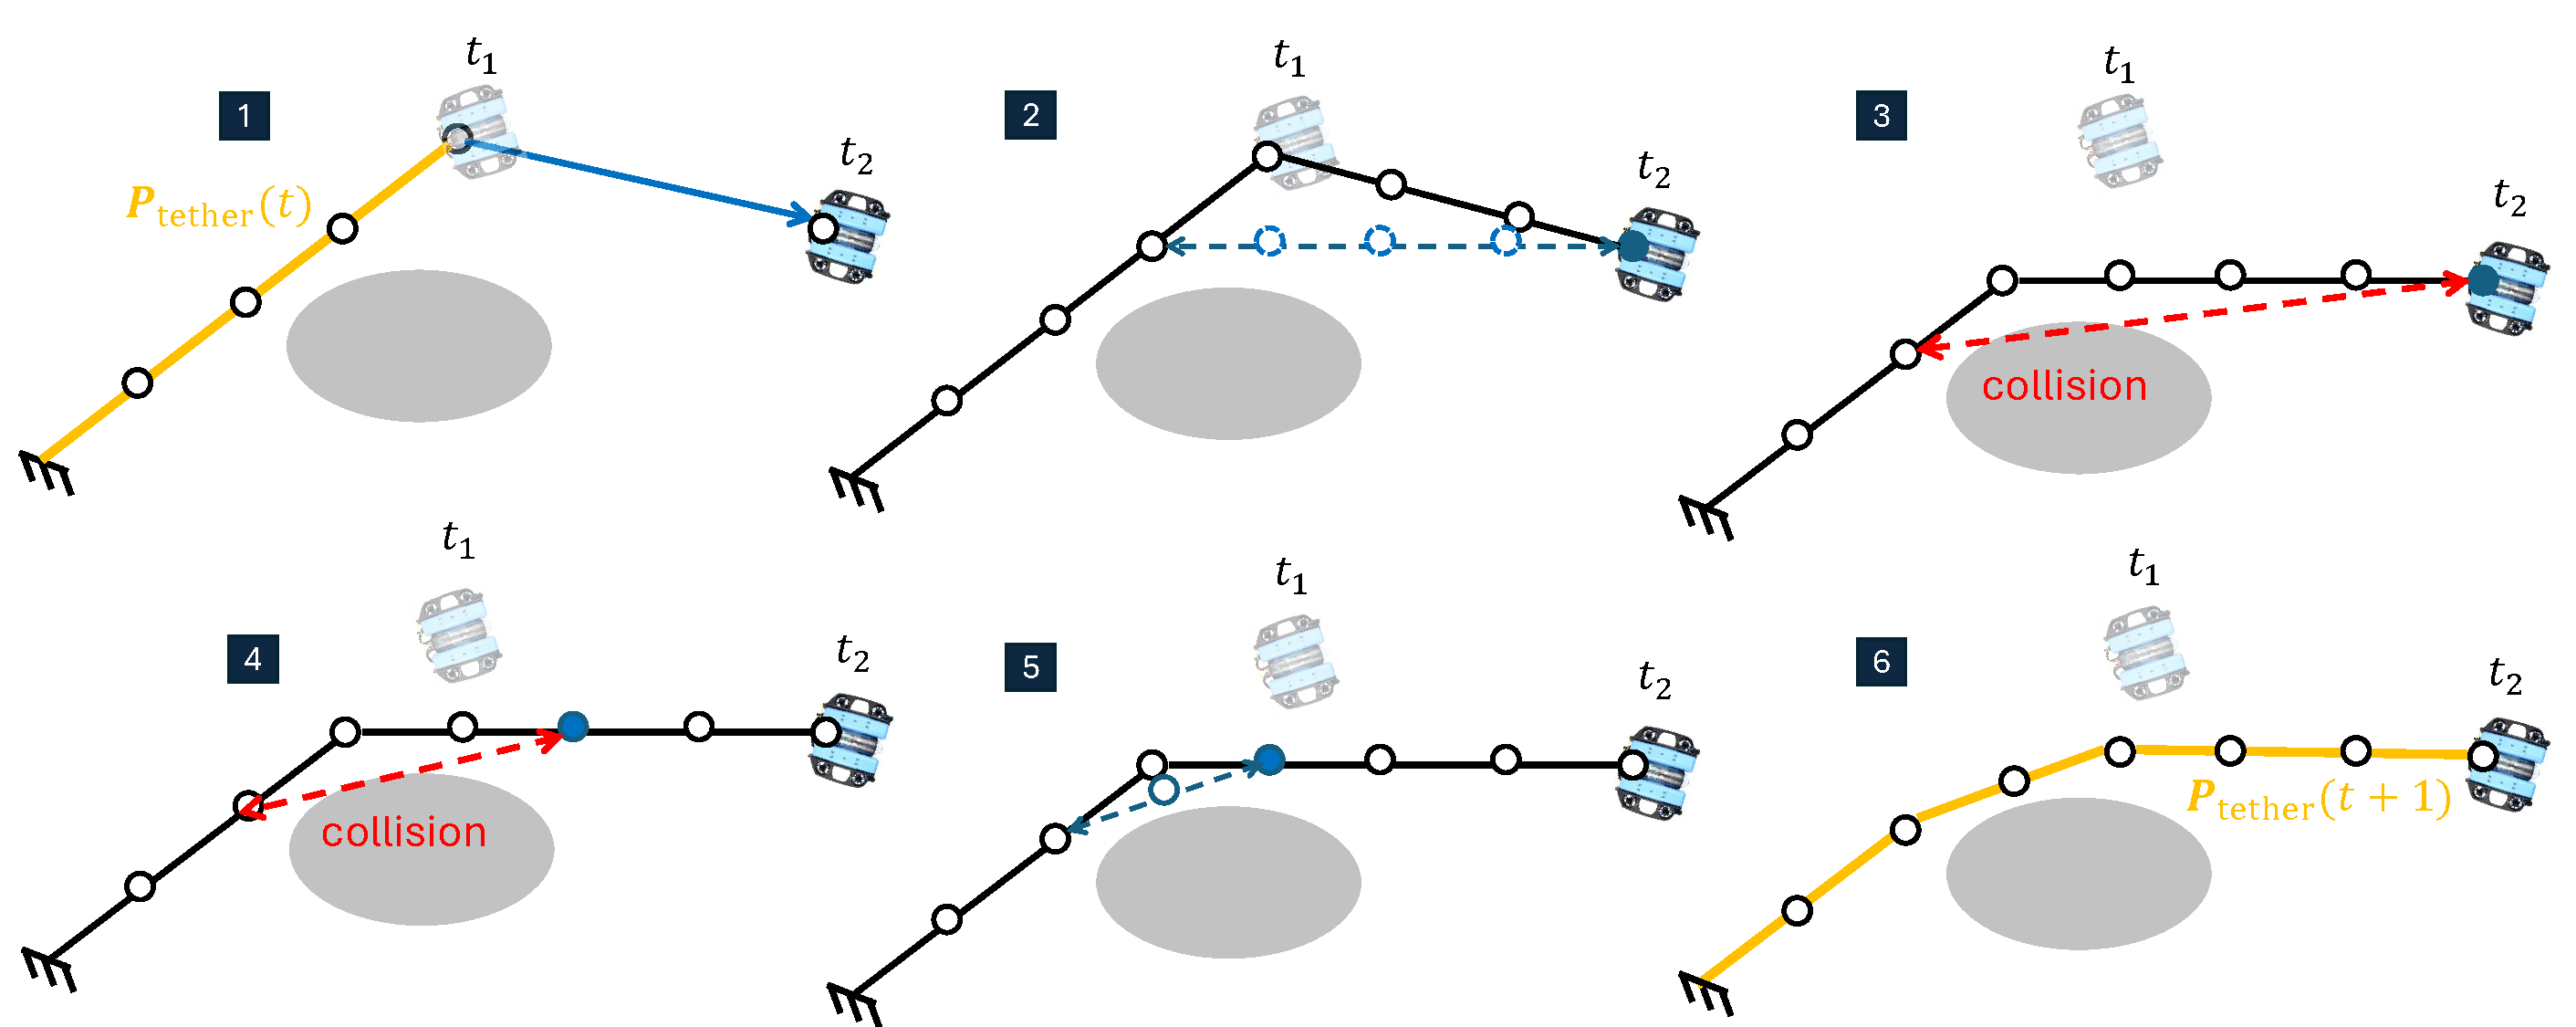
\includegraphics[width=1\linewidth]{EA-Planner/figures/tether_model.pdf}
    \caption{Tether shortcutting during \ac{ROV} motion from \( t_1 \) to \( t_2 \). (1) Initial tether with new \ac{ROV} position \( \mathbf{p}_{\text{rov}} \) appended; (2) Successful shortcut from the end node; (3) Collision encountered when attempting further shortcutting, prompting move to the next node; (4) Another collision detected from the new node; (5) Successful shortcut from a subsequent node; (6) Final tether configuration (yellow) after applying all feasible shortcuts.}
    \label{fig:tether}
\end{figure*}



%%%%%%%%%%%%%%%%%%%%%%%%%%%%%%%%%%%%%%%%%%
%%%%%%  Tether Model Algorithm  %%%%%%%%%
%%%%%%%%%%%%%%%%%%%%%%%%%%%%%%%%%%%%%%%%%%


\begin{algorithm}[H]
%\SetAlgoLined
\LinesNotNumbered  % Disable line numbers

\SetKwInOut{Input}{Require}
\SetKwInOut{Output}{Return}
\Input{
ROV position $\mathbf{p}_{rov}(t)$, 
Tether path $\mathbf{P}^{tether}(t)$, 
SDF map $\mathcal{M}_{sdf}$, 
parameters: $\delta_{n}$
}
\Output{Taut-tether at $t+1$ : $\mathbf{P}^{tether}(t+1)$}
\BlankLine

\tcp{Extend tether path to include the current ROV position as the endpoint}
Append $\mathbf{p}_{rov}(t)$ to $\mathbf{P}^{tether}(t).end()$\;

\tcp{Iteratively attempt to shortcut path segments by skipping intermediate nodes}

\For{$i \gets len(\mathbf{P}^{tether}(t)) - 2$ \textbf{to} $1$}{
    \For{$j \gets i+1$ \textbf{to} $len(\mathbf{P}^{tether}(t)) - 1$}{
        \tcp{Check if shortcutting the path is valid between nodes $i$ and $j$}
        \If{checkshortcut($\mathbf{P}^{tether}(t), i, j$)}{
            \tcp{Replace intermediate nodes between $i$ and $j$ with straight segment}
            ReplaceIntermediateNodes($\mathbf{P}^{tether}(t)$, $i$, $j$, $\delta_{n}$)\;
        }
        \Else{
            \If{not CheckLineOfSight($\mathcal{M}_{sdf}$, $\mathbf{P}^{tether}(t)$)}{
                \tcp{Line of sight is blocked by obstacle, stop shortcutting}
                \textbf{break}\;
            }
            \If{isInCollision($\mathcal{M}_{sdf}$, $\mathbf{P}^{tether}(t)[j]$)}{
                \tcp{Pull node towards tether end}
                PullNode($\mathbf{P}^{tether}(t)[j]$, $\mathbf{P}^{tether}(t).end()$, $\delta_{n}$)\;
            }
        }
    }
}
\Return{$\mathbf{P}^{tether}(t+1)$}\;
\caption{Taut-Tether Model}
\label{alg:tether_optimization}
\end{algorithm}

%%%%%%%%%%%%%%%%%%%%%%%%%%%%%%%%%%%%%%%%%%
%%%%%%%%%%%%%%%%%%%%%%%%%%%%%%%%%%%%%%%%%%
%%%%%%%%%%%%%%%%%%%%%%%%%%%%%%%%%%%%%%%%%%


If the shortcut is obstructed or the endpoint node \( p_j(t) \) is in collision, the model applies a pulling operation. This simulates disentanglement by moving \( p_j(t) \) incrementally toward the tether endpoint \( p_{N+1}(t) \), ensuring the new configuration remains collision-free. This iterative process continues until no further shortcutting or pulling is possible, resulting in an updated, taut, and obstacle-free tether path \( \mathbf{P}^{tether}(t+1) \). An example of the shortcutting operation is illustrated in Fig.~\ref{fig:tether}.


%%%%%%%%%%%%%%%%%%%%%%%%%%%
%%%%%%%%%%%%%%%%%%%%%%%%%%%
%%%%%%% PLANNER %%%%%%%%%
%%%%%%%%%%%%%%%%%%%%%%%%%%
%%%%%%%%%%%%%%%%%%%%%%%%%%


\section{Real-Time Entanglement-Aware Path Planner}
\label{sec:planner}

In this section, we present the real-time entanglement-aware path planner, a local planner designed to handle real-time entagelemnt-free path finding for autonomous system navigating operating with a tether. The planner runs in an online manner, continuously monitoring the tether configuration and adapting the \ac{ROV}'s path to avoid exceeding the maximum allowable tether length, \( L_{\text{max}} \), while ensuring safe, collision-free motion towards a sequence of reference waypoints.

At each time step \( t \), the planner utilizes the current estimated tether configuration  $\mathbf{P}^{tether}(t)$. The planner also maintains a list of reference waypoints \( \mathbf{W} = \{\mathbf{p}_{\text{waypoint}}(k)\}_{k=1}^{M} \), where \( \mathbf{p}_{\text{waypoint}}(k) \in \mathbb{R}^3 \) denotes the \( k \)-th target waypoint. The current tether length \( L_{\text{tether}}(t) \) is computed by summing the Euclidean distances between consecutive tether points, i.e., \( L_{\text{tether}}(t) = \sum_{i=1}^{N-1} \| p_i(t) - p_{i+1}(t) \| \), and is subsequently compared to the predefined maximum allowable length \( L_{\text{max}} \), to activate the re-planner.

\subsection{Nominal Operation}
If the tether length constraint is satisfied, i.e., \( L_{\text{tether}}(t) \leq L_{\text{max}} \), the planner operates in its nominal mode. It identifies the next reference waypoint \( \mathbf{p}_{\text{waypoint}}(k) \) from the list \( \mathbf{W} \) that has not yet been reached and directs the \ac{ROV} controller towards it. The system proceeds sequentially through the waypoints as long as the tether constraint remains satisfied.



\subsection{Entanglement Avoidance Strategy}
If the tether length exceeds the maximum allowable limit, \( L_{\text{tether}}(t) > L_{\text{max}} \), the entanglement avoidance strategy is activated. This strategy aims to guide the \ac{ROV} along a temporary recovery path to de-tangle the tether before resuming navigation towards the original target waypoint.

The planner initiates a search for a suitable recovery path by iteratively evaluating potential de-tangle paths based on the current tether configuration \( \mathbf{P}^{tether}(t) \). Starting from the \ac{ROV}'s end of the tether (node \( p_{N-1}(t) \)) and moving backward towards the anchor point \( p_1(t) \), the planner considers each node \( p_i(t) \) as a potential pivot point. For each \( i \), a candidate alternative trajectory is implicitly generated, consisting of the segment from the \ac{ROV} back to \( p_i(t) \) followed by a newly planned path segment from \( p_i(t) \) to the current target waypoint \( \mathbf{p}_{\text{waypoint}}(k) \). The planner computes the estimated length of this candidate alternative tether configuration.

A recovery path is selected based on length criteria: the planner seeks a pivot point \( p_i(t) \) such that the corresponding alternative path length is significantly shorter than \( L_{\text{max}} \) (e.g., \( < 0.7 L_{\text{max}} \)) and offers substantial improvement compared to alternatives generated using nearby pivot points (e.g., \( p_{i-3}(t) \)). Once such an index \( i \) is found, the recovery path segment \( \mathbf{P}_{\text{recovery}} \) is defined as the portion of the current tether from the \ac{ROV} back to a point slightly further back along the tether, specifically \( p_{i+2}(t) \). This segment represents the initial trajectory the \ac{ROV} must follow to begin resolving the entanglement. If no suitable recovery path is found during the backward search, a direct path from the \ac{ROV}'s current position to the goal waypoint is generated as a fallback. This recovery path search process is illustrated in Fig. \ref{fig:planner_search}.  











\subsection{Recovery Path Refinement and Execution}
The initially selected recovery path \( \mathbf{P}_{\text{recovery}} \) undergoes further refinement to enhance safety and smoothness before execution. This involves several steps:
\begin{enumerate}
    \item \textbf{Centroid Offsetting:} Points along \( \mathbf{P}_{\text{recovery}} \) are pushed slightly outwards, away from the path's geometric centroid, to increase clearance from potential obstacles near the path's center.
    \item \textbf{Random Sampling Perturbation:} Points are locally perturbed by sampling in random directions, seeking nearby collision-free states to potentially escape minor constraint violations or local minima.
    \item \textbf{Polynomial Smoothing:} A polynomial function (e.g., 3rd order) is fitted to segments of the path to generate a smoother trajectory, reducing sharp turns and improving dynamic feasibility.
\end{enumerate}
The resulting refined path is denoted as \( \mathbf{P}_{\text{safe}} \). The planner then checks if \( \mathbf{P}_{\text{safe}} \) is collision-free using the state validity checker. If the entanglement strategy is active and \( \mathbf{P}_{\text{safe}} \) is valid, the controller is directed to follow points sequentially along \( \mathbf{P}_{\text{safe}} \). Once the \ac{ROV} reaches the end of \( \mathbf{P}_{\text{safe}} \), the entanglement avoidance strategy is deactivated, and the planner reverts to nominal operation, targeting the next waypoint from the original list \( \mathbf{W} \). If \( \mathbf{P}_{\text{safe}} \) is found to be invalid (e.g., due to collisions introduced during refinement), the system continues targeting the original waypoint \( \mathbf{p}_{\text{waypoint}}(k) \), relying on lower-level collision avoidance or requiring further planning cycles. 

The core logic can be summarized in the following algorithms. Algorithm~\ref{alg:main_loop} outlines the main planning cycle, Algorithm~\ref{alg:search_alternative} details the search for the recovery path, and Algorithm~\ref{alg:refine_path} describes the path refinement process.




%%%%%%%%%%%%%%%%%%%%%%%%%%%
%%%%% REACT Planner %%%%%%
%%%%%%%%%%%%%%%%%%%%%%%%%%%
\begin{algorithm}[t]
\LinesNotNumbered  % Disable line numbers

\SetKwInOut{Input}{Input}
\SetKwInOut{Output}{Return}
\Input{
Waypoints $\mathbf{W}$, 
Maximum tether length $L_{\max}$, 
Current tether configuration $\mathbf{P}^{tether}(t)$, 
Current ROV position $\mathbf{p}_{\text{rov}}(t)$, 
Current waypoint index $k$, $d_{thresh}$}

\Output{Target point for controller $\mathbf{p}_{\text{target}}$}
\BlankLine

Compute $L_{\text{tether}}(t)$ from $\mathbf{P}^{tether}(t)$\; \tcp{Measure current tether length}

\If{$L_{\text{tether}}(t) > L_{\max}$ \textbf{and not} finding\_safe\_path}{
    finding\_safe\_path $\gets$ True\; \tcp{Activate recovery mode}
    $\mathbf{P}_{\text{recovery}} \gets \text{SearchAlternativePath}(\mathbf{P}^{tether}(t), \mathbf{W}[k], L_{\max})$\; \tcp{Find a path to waypoint within tether limits}
    $\mathbf{P}_{\text{safe}} \gets \text{RefineRecoveryPath}(\mathbf{P}_{\text{recovery}})$\; \tcp{Optimize the recovery path}
    path\_is\_safe $\gets \text{CheckPathValidity}(\mathbf{P}_{\text{safe}})$\; \tcp{Check if recovery path is valid}
    safe\_path\_index $\gets 0$\; \tcp{Start from the beginning of the recovery path}
}

\If{finding\_safe\_path \textbf{and} path\_is\_safe}{
    $\mathbf{p}_{\text{target}} \gets \text{GetPointAlongPath}(\mathbf{P}_{\text{safe}}, \text{safe\_path\_index})$\; \tcp{Get current target from recovery path}
    \If{$\|\mathbf{p}_{\text{rov}}(t) - \mathbf{p}_{\text{target}}\| < d_{thresh}$}{
        safe\_path\_index $\gets$ safe\_path\_index + 1\; \tcp{Advance to next point if target is reached}
    }
    \If{safe\_path\_index $\ge$ $|\mathbf{P}_{\text{safe}}|$}{
        finding\_safe\_path $\gets$ False\; \tcp{Recovery complete}
        $\mathbf{p}_{\text{target}} \gets \mathbf{W}[k]$\; \tcp{Resume wp tracking}
    }
}
\Else{
    finding\_safe\_path $\gets$ False\; \tcp{Reset recovery if no valid path}
    $\mathbf{p}_{\text{target}} \gets \mathbf{W}[k]$\; \tcp{Default to current waypoint}

    \If{$\|\mathbf{p}_{\text{rov}}(t) - \mathbf{p}_{\text{target}}\| < d_{thresh}$}{
         $k \gets k + 1$\; \tcp{Advance to next waypoint}
    }
}
\Return{$\mathbf{p}_{\text{target}}$}\;
\caption{Real-time Entanglement-Aware Path Planning}
\label{alg:main_loop}
\end{algorithm}



%%%%%%%%%%%%%%%%%%%%%%%%%
%%%% Figure : Planner search 
%%%%%%%%%%%%%%%%%%%%%%%%
%%%%%%%%%%%%%%%%%%%%%%%%
\begin{figure*}[t]
    \centering
    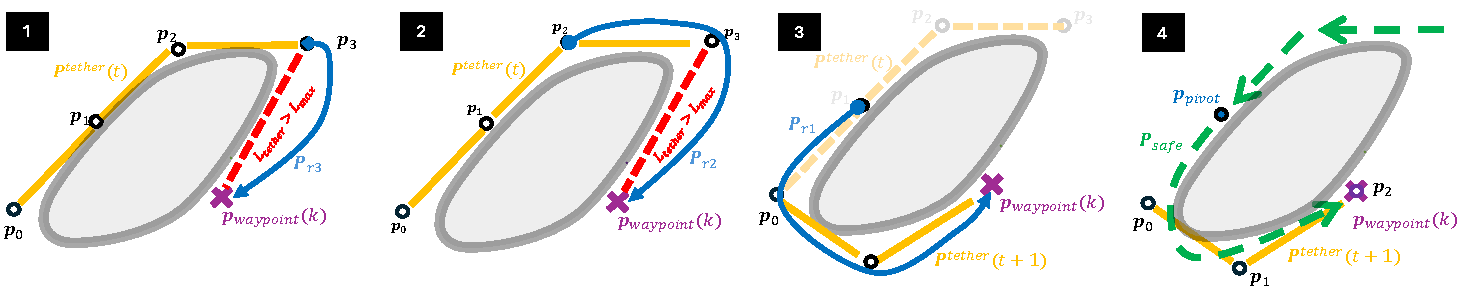
\includegraphics[width=\textwidth]{EA-Planner/figures/planner.pdf}
    \caption{Recovery path search process: 
    (1) Following the path from node \( \mathbf{p}_3 \), denoted as \( \mathbf{P}_{r_3} \), causes the tether length \( L_{\text{tether}} \) to exceed the maximum allowed length \( L_{\text{max}} \); 
    (2) a backward recovery search is initiated from node \( \mathbf{p}_2 \) along the tether trajectory \( \mathbf{P}_{tether}(t) \), but the resulting path yields no improvement in tether length; 
    (3) continuing the search further back to node \( \mathbf{p}_1 \) leads to a feasible path and an updated, valid tether configuration; 
    (4) the final planned safe path \( \mathbf{P}_{safe} \) (green) satisfies the tether constraint (\( L_{\text{tether}} \leq L_{\text{max}} \)), ensuring an entanglement-free configuration.}
    \label{fig:planner_search}
\end{figure*}
%%%%%%%%%%%%%%%%
%%%%%%%%%%%%%%%%



%%%%%%%%%%%%%%%%%%%%%%%%%%%%%%%%%%%%%%%%%%
%%%%%%%%%%%%%%%%%%%%%%%%%%%%%%%%%%%%%%%%%%
%%%%%%%%%%%%%%%%%%%%%%%%%%%%%%%%%%%%%%%%%%


%%%%%%%%%%%%%%%%%%%%%%%%%%%%%%%%%
%% Recovery Path  Algorithm %%%
%%%%%%%%%%%%%%%%%%%%%%%%%%%%%%%%%

\begin{algorithm}[H]
\SetKwInOut{Input}{Require}
\SetKwInOut{Output}{Return}
\Input{
Current tether $\mathbf{P}(t)$,
Goal waypoint $\mathbf{p}_{\text{goal}}$,
Maximum length $L_{\max}$
}
\Output{Recovery path segment $\mathbf{P}_{\text{recovery}}$}
\BlankLine
best\_path $\gets$ None\;
prev\_len $\gets \infty$\;
found\_suitable $\gets$ False\;
\For{$i \gets |\mathbf{P}(t)| - 3$ \textbf{downto} 3}{
    $\mathbf{P}_{\text{candidate}} \gets \text{GenerateCandidatePath}(i, \mathbf{P}(t), \mathbf{p}_{\text{goal}})$\;
    $L_{\text{candidate}} \gets \text{ComputeLength}(i, \mathbf{P}(t), \mathbf{P}_{\text{candidate}})$\;
    \If{$L_{\text{candidate}} < 0.7L_{\max}$} %\textbf{and} $L_{\text{candidate}} < 0.65 \cdot \text{prev\_len}$}
    {
         best\_path $\gets \text{ExtractSegment}(i+2, \mathbf{P}(t))$\;
         found\_suitable $\gets$ True\;
         \textbf{break}\;
    }
    prev\_len $\gets \text{ComputeLength}(i-3, \mathbf{P}(t), \text{GeneratePath}(i-3, \mathbf{P}(t), \mathbf{p}_{\text{goal}}))$\;
}
\If{\textbf{not} found\_suitable}{
    $\mathbf{p}_{\text{rov}} \gets \mathbf{P}(t)[|\mathbf{P}(t)|-1]$\; \tcp{Fallback}
    $\mathbf{P}_{\text{recovery}}$ $\gets \text{PlanShortestPath}(\mathbf{p}_{\text{rov}}, \mathbf{p}_{\text{goal}})$\;
}
\Return{$\mathbf{P}_{\text{recovery}}$}\;
\caption{Search Alternative Recovery Path}
\label{alg:search_alternative}
\end{algorithm}

%%%%%%%%%%%%%%%%%%%%%%%%%%%%%%%%%%%%%%%%%%
%%%%%%%%%%%%%%%%%%%%%%%%%%%%%%%%%%%%%%%%%%
%%%%%%%%%%%%%%%%%%%%%%%%%%%%%%%%%%%%%%%%%%

%%%%%%%%%%%%%%%%%%%%%%%%%%%
%% Refine Path  Algorithm
%%%%%%%%%%%%%%%%%%%%%%%%%%%
\begin{algorithm}[H]
\LinesNotNumbered  % Disable line numbers
\SetKwInOut{Input}{Input}
\SetKwInOut{Output}{Return}
\Input{
    Recovery path $\mathbf{P}_{\text{recovery}}$;\\
    Offset distance $\delta_{\text{offset}}$;\\
    Sampling distance $\delta_{\text{sample}}$
}
\Output{Refined safe path $\mathbf{P}_{\text{safe}}$}
\BlankLine
$\mathbf{P}_{\text{offset}} \gets \text{PopTetherCentroid}(\mathbf{P}_{\text{recovery}}, \delta_{\text{offset}})$\;
\\
$\mathbf{P}_{\text{sampled}} \gets \text{PopPathSample}(\mathbf{P}_{\text{offset}}, \delta_{\text{sample}})$\;
\\
$\mathbf{P}_{\text{safe}} \gets \text{SmoothPathWithPolynomial}(\mathbf{P}_{\text{sampled}})$\;
\\
\Return{$\mathbf{P}_{\text{safe}}$}\;
\caption{Refine Recovery Path}
\label{alg:refine_path}
\end{algorithm}


%%%%%%%%%%%%%%
%%%%%%%%%%%%%%
%%%%%%%%%%%%%%